%%%%%%%%%%%%%%%%%%%%%%%%%%%%%%%%%%%%%%%%%%%%%%%%%%%%%%%%%%%%%%%%%%%%%%%%%%%%%%%%
\chapter{Проектирование генератора систем инструментирования}
%%%%%%%%%%%%%%%%%%%%%%%%%%%%%%%%%%%%%%%%%%%%%%%%%%%%%%%%%%%%%%%%%%%%%%%%%%%%%%%%

В данном разделе описывается процесс разработки расширяемого генератора систем инструментирования исходного текста программ.

%%%%%%%%%%%%%%%%%%%%%%%%%%%%%%%%%%%%%%%%%%%%%%%%%%%%%%%%%%%%%%%%%%%%%%%%%%%%%%%%
\section{Принцип работы системы инструментирования}
%%%%%%%%%%%%%%%%%%%%%%%%%%%%%%%%%%%%%%%%%%%%%%%%%%%%%%%%%%%%%%%%%%%%%%%%%%%%%%%%

Как уже было рассмотрено ранее, инструментирование заключается в выполнении специфических модификаций/трансформаций, выполняемых над некоторым программным кодом.
Согласно этой формулировке, процесс инструментирования можно организовать следующим образом:
\begin{itemize}[noitemsep]
  \item на входе системы имеется источник исходного текста на некотором языке программирования;
  \item имеется механизм, способный осуществить необходимые трансформации над текстом;
  \item на выходе генерируется инструментированный текст на том же самом языке программирования.
\end{itemize}

Для построения гибкой системы из приведенной последовательности необходимо ввести промежуточный артефакт в виде некоторого описания требуемых трансформаций.

В соответствии с этим была составлена обобщенная схема работы генератора систем инструментирования исходных текстов программ, изображенная на рисунке~\ref{fig:layout_artifacts}, с позиции обрабатываемых и производимых артефактов, таких как файлы и аргументы командной строки (параметры запуска).

\begin{figure}[!h]
	\centering
	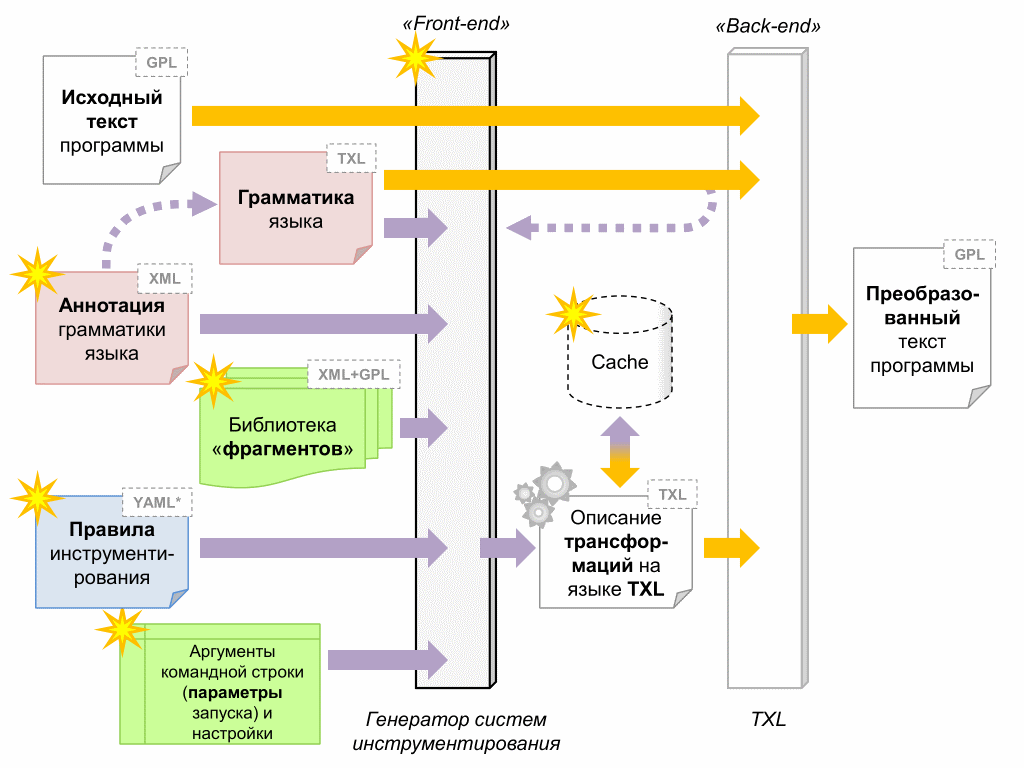
\includegraphics[width=3.7in]{layout_artifacts}
	\caption{Cхема работы системы. Артефакты.}
	\label{fig:layout_artifacts}
\end{figure}

На схеме изображены следующие артефакты, необходимые для решения задачи инструментирования, которые являются \underline{входными} для связки ``генератор + система трансформаций'':
\begin{itemize}[noitemsep]
  \item текст программы, инструментирование которой необходимо выполнить;
  \item описание грамматики выбранного в качестве целевого языка программирования, на котором написан исходный текст этой программы;
  \item аннотация грамматики выбранного языка программирования;
  \item описание пользовательских правил инструментирования;
  \item фрагменты исходных текстов на выбранном языке программирования, вставку которых необходимо выполнить;
  \item дополнительные необязательные параметры запуска системы и переменные среды исполнения.
\end{itemize}

\underline{Промежуточным} артефактом работы генератора систем инструментирования исходного текста программ является описание трансформаций, которые необходимо выполнить над конкретным входным файлом с текстом программы с учетом предоставленной грамматики целевого языка программирования.

\underline{Выходным} артефактом является текст программы на целевом языке программирования, над которым были выполнены необходимые трансформации.

Важно отметить, что на данной схеме не показано интерактивное взаимодействие с пользователем, например выводимые сообщения об успешном инструментировании или встреченных ошибках.

Рассмотрим некоторые артефакты и процессы, в которых они участвуют, более подробно с точки зрения возможных способов реализации.

%%%%%%%%%%%%%%%%%%%
\subsection{Аннотация грамматики языка}
%%%%%%%%%%%%%%%%%%%

Из специфики задачи очевидно существование некоторого множества элементарных операций, которые необходимо выполнять многократно при осуществлении инструментирования некоторой кодовой базы, содержащей большое количество файлов, содержащих текст на целевом языке программирования.
Исходя из этого, разумным решением является выделение некоторых из этих операций в качестве аннотации к грамматике целевого ЯП, а остальных операций -- в виде создаваемых пользователями высокоуровневых декларативных описаний требуемого процесса инструментирования.

Рассмотрим более подробно возможную организацию аннотации к грамматике некоторого языка программирования.

Аннотация грамматики предназначается для сокращения множества $G$ всех узлов бесконечного множества деревьев разбора, описываемых грамматикой целевого ЯП в виде графовой структуры, в данном случае -- с помощью языка утилиты TXL, до множества транзитивно связанных узлов $G^* \subset G$.

Одними из наиболее важных задач, решаемых составлением аннотации являются:

\begin{itemize}[noitemsep]
  \item описание всех синтаксических конструкций целевого языка программирования, которые являются наиболее существенными с точки зрения составителя аннотации, с учетом потребностей конечного пользователя в лице составителя правил инструментирования;
  \item описание всех необходимых потенциальному конечному пользователю точек инструментирования для всех выбранных синтаксических конструкций;
  \item императивное описание алгоритма инструментирования каждой точки инструментирования.
\end{itemize}

Помимо этого, аннотация \textit{должна} являться для пользователя упрощенной схемой (подсказкой) иерархии типов узлов дерева разбора, в которой отображены только наиболее важные понятия языка программирования, для которого выполняется инструментирование, такие как \textit{класс}, \textit{метод}, \textit{оператор ветвления}, \textit{цикл со счетчиком} и т.п.

Для описания точек инструментирования, а именно, точного указания места вставки среди уже существующих, или вновь создаваемых, узлов конкретного дерева разбора можно выделить два основных подхода:

\begin{enumerate}[noitemsep]
  \item использовать некоторую относительную или абсолютную систему адресации, например, подобную XPath~\cite{xpath};
  \item использовать текстовый шаблон со специальным образом обозначенными заполнителями.
\end{enumerate}
\nomenclature{XPath}{XML Path Language -- язык запросов к XML документам.}

Использование текстового шаблона позволит в некоторой степени, за счет внутренних особенностей утилиты TXL~\cite{txl-book}, упростить создание новых и промежуточных узлов в модифицируемом дереве разбора.

Поскольку аннотации включают в себя
шаблоны выбранных синтаксических конструкций целевого языка программирования вместе с 
алгоритмами, императивно описывающими процесс инструментирования всех перечисленных точек инструментирования,
необходимо перечислить требования к языку, используемому для описания аннотаций:

\begin{itemize}[noitemsep]
  \item текстовый вид представления данных;
  \item поддержка иерархических структур данных;
  \item возможность использования любых символьных последовательностей, включая используемые самим языком описания, путем экранирования специальных символов;
  \item возможность внесения дальнейших расширений и улучшений посредством добавления новых конструкций и атрибутов.
\end{itemize}

Приведенным выше требованиям соответствуют такие языки как, например, JSON~\cite{json}, YAML~\cite{yaml} и XML~\cite{xml}.
\nomenclature{JSON}{JavaScript Object Notation -- язык описания объектов языка JavaScript.}
\nomenclature{XML}{eXtensible Markup Language -- расширяемый язык разметки.}
\nomenclature{YAML}{Yet Another Markup Language, YAML Ain't Markup Language --  формат сериализации данных.}
Поскольку язык XML удовлетворяет всем приведенным требованиям, является общеупотребимым (имея средства разбора для широкого спектра языков программирования) и применяется как часть реализации утилиты TXL~\cite{txl-freetxl}, было принято решение об использовании этого языка для описания аннотаций грамматик.

%%%%%%%%%%%%%%%%%%%
\subsection{Фрагменты программного кода}
%%%%%%%%%%%%%%%%%%%

Для каждого из добавляемых конечными пользователями фрагментов исходных текстов необходимо иметь возможность автоматизировано определить следующие ключевые характеристики:

\begin{itemize}[noitemsep]
  \item название фрагмента;
  \item текст фрагмента;
  \item язык программирования, на котором написан текст фрагмента;
  \item возможные зависимости текущего фрагмента от других фрагментов;
  \item множество используемых в тексте фрагмента текстовых заполнителей, если фрагмент параметризуем.
\end{itemize}

Таким образом, приведенные выше доводы, касательно организации пользовательского описания аннотаций грамматик различных целевых языков программирования, применимы и к способам хранения и организации добавляемых фрагментов исходного кода.

%%%%%%%%%%%%%%%%%%%
\subsection{Правила инструментирования}
%%%%%%%%%%%%%%%%%%%

Как уже было представлено ранее в разделе 2, имеется необходимость отдельного от аннотации декларативного описания пользовательских правил инструментирования.
Для решения этой задачи существуют следующие подходы:
\begin{itemize}[noitemsep]
  \item выбор существующего императивного языка программирования;
  \item выбор существующего декларативного языка программирования;
  \item создание нового узкоспециализированного языка;
\end{itemize}

Применение существующего императивного ЯП подразумевает создание некоторого декларативного API и набора сущностей, управление которыми должен осуществлять конечный пользователь, что замедляет рабочий процесс разработчика (пользователя).
\nomenclature{API}{Application Programming Interface -- интерфейс программирования приложений.}

Применение существующего декларативного языка ограничено отсутствием расширяемых чисто декларативных языков программирования, предполагающих добавление или удаление какой-либо функциональности.

Исходя из этого, необходимо разработать небольшой узкоспециализированный язык описания пользовательских правил, который должен в том или ином виде позволять пользователю осуществлять следующие действия:
\begin{itemize}[noitemsep]
  \item перечислять интересующих пользователя контекстов инструментирования;
  \item перечислять используемых в данном наборе правил фрагментов исходных текстов, с указанием параметров, если таковые требуются согласно тексту используемого фрагмента;
  \item описывать уточнение контекста инструментирования с применением ключевых слов языка программирования и текстовых шаблонов, если таковые требуются для целей уточнения контекста согласно решаемой пользователем задачи;
  \item указывать конкретные точки инструментирования каким-либо способом;
  \item объявлять пользовательские переменные;
  \item иметь поддержку именования правил инструментирования.
\end{itemize}

%%%%%%%%%%%%%%%%%%%
\subsection{Пользователи системы}
%%%%%%%%%%%%%%%%%%%

На рисунке~\ref{fig:layout_users} приведена схема работы системы инструментирования с позиции взаимодействия пользователей и системы как части производственного процесса создания и отладки некоторого программного продукта.

\begin{figure}[!h]
	\centering
	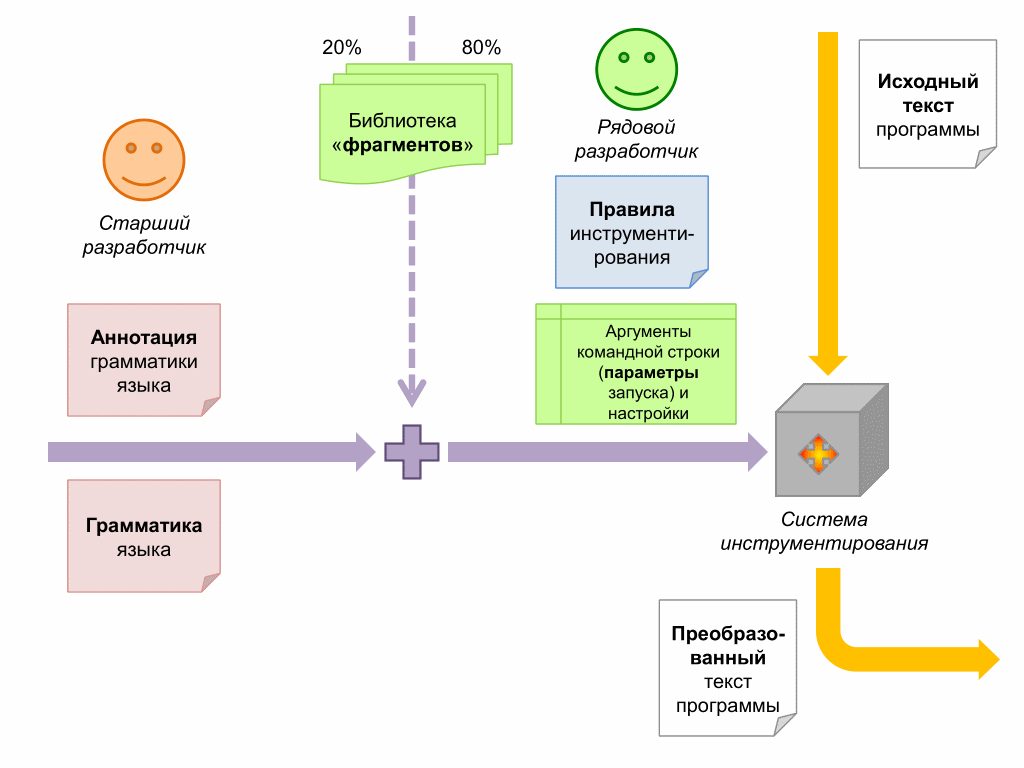
\includegraphics[width=4.2in]{layout_users}
	\caption{Cхема работы системы. Пользователи.}
	\label{fig:layout_users}
\end{figure}

С учетом того факта, что при выполнении инструментирования производится множество повторяющихся элементарных действий, которые были вынесены отдельно в виде аннотации грамматики, по схожему принципу были разделены обязанности конечного пользователя в виде двух ролей:
\begin{itemize}[noitemsep]
  \item Разработчик грамматики -- более опытный пользователь, в лице старшего разработчика, в задачи которого входит:
    \begin{itemize}[noitemsep]
      \item описание грамматики целевого языка программирования;
      \item составление аннотации к грамматике;
      \item отладка аннотации и грамматики;
      \item составление примеров фрагментов на целевом языке программирования.
    \end{itemize}

  \item Составитель правил инструментирования -- конечный пользователь, в лице рядового разработчика, в задачи которого входит:
    \begin{itemize}[noitemsep]
      \item составление правил инструментирования;
      \item создание и пополнение библиотеки фрагментов исходных текстов на целевом языке;
      \item применение системы инструментирования к исходным текстам какой-либо программной системы.
    \end{itemize}
\end{itemize}

Исходя из задач, решаемых разными пользователями системы, можно выделить следующий неполный набор компетенций для разных групп пользователей системы:

\begin{itemize}[noitemsep]
  \item Разработчик грамматики и аннотации:
    \begin{itemize}[noitemsep]
      \item иметь опыт применения языков, предложенных выше, для описания аннотации;
      \item понимать базовые принципы работы с графовыми и древовидными структурами данных;
      \item иметь опыт успешной разработки и отладки грамматик или правил трансформации на языке TXL или подобных;
      \item иметь опыт применения целевого языка программирования для решения производственных задач (разработки, тестирования и отладки программных или программно-аппаратных систем).
    \end{itemize}

  \item Составитель правил инструментирования:
    \begin{itemize}[noitemsep]
      \item понимать базовые принципы работы с графовыми и древовидными структурами данных;
      \item иметь опыт применения целевого языка программирования для решения производственных задач (разработки, тестирования и отладки программных или программно-аппаратных систем).
    \end{itemize}
\end{itemize}

%%%%%%%%%%%%%%%%%%%
\subsection{Выходные артефакты генератора}
%%%%%%%%%%%%%%%%%%%

Наиболее значимым и единственным, согласно рисунку~\ref{fig:layout_artifacts}, выходным артефактом генератора систем инструментирования исходного кода программ является текстовое описание трансформаций на языке TXL в виде некоторого файла.
Поскольку проектируемый генератор может использоваться как часть процесса сборки некоторого промышленного программного обеспечения, которое имеет большой объем кодовой базы, можно сделать заключение о необходимости обеспечить разумный уровень сокращения повторяющихся ресурсозатратных действий.

Наиболее ресурсозатратными действиями при работе системы инструментирования будут являться следующие:
\begin{itemize}[noitemsep]
  \item чтение каких-либо данных из файлового хранилища (жесткие диски, RAID-массивы жестких дисков);
  \item запись каких-либо данных в файловое хранилище;
  \item анализ и предобработка считанных данных;
  \item обработка и синтез выходных данных во временной памяти;
  \item запуск и ожидание других процессов операционной системы.
\end{itemize}
\nomenclature{RAID}{Redundant Array of Independent Disks -- технология виртуализации данных для объединения физических дисковых устройств.}

С учетом относительного времени, которое необходимо для выполнения различных операций, приведенный список можно упорядочить следующим образом (меньше номер -- лучше):
\begin{enumerate}[noitemsep]
  \item анализ и предобработка считанных данных;
  \item обработка и синтез выходных данных во временной памяти;
  \item чтение данных из файлового хранилища;
  \item запись данных в файловое хранилище;
  \item запуск и ожидание других процессов.
\end{enumerate}

Для простоты, примем время работы пунктов $1$ и $2$ одинаковым.

С учетом полученных результатов, рассмотрим более детально предполагаемый процесс инструментирования, изображенный на рисунке~\ref{fig:layout_artifacts}, уделяя внимание наиболее ресурсоемким выполняемым операциям.

Для генерации промежуточного описания трансформаций на языке TXL, генератору требуется выполнить \textbf{чтение} из файлового хранилища следующих артефактов:
\begin{itemize}[noitemsep]
  \item грамматика целевого языка программирования;
  \item аннотация к грамматике;
  \item пользовательские правила инструментирования;
  \item несколько фрагментов из библиотеки фрагментов (зависимость от пользовательского описания, $N$).
\end{itemize}

Таким образом, генератор систем инструментирования должен выполнить $3 + N$ раздельных чтений из файлового хранилища, чтобы впоследствии выполнить \textbf{запись} в файловое хранилище промежуточного описания трансформаций и \textbf{запустить} утилиту TXL, которая в свою очередь выполнит несколько (минимум $3$, как видно на рисунке~\ref{fig:layout_artifacts}) чтений и, как минимум, одну запись, в зависимости от сложности и структуры грамматики целевого языка программирования, для непосредственного инструментирования обрабатываемого исходного текста программы как часть завершающего этапа.

Из рассмотрения были исключены динамически загружаемые разделяемые модули и библиотеки программного кода, потому как они являются частью среды исполнения и позволяют существенно снизить время и стоимость производства программных продуктов различного назначения, применяемых в пространстве пользователя (в терминах операционной системы).
Значительно уменьшить их эффект на время работы общей системы инструментирования (совместно с генератором) можно посредством создания однократно запускаемого процесса-сервиса (``демона'' в терминах ОС GNU Linux), который выполнял основную часть работ, получая указания от легковесного многократно запускаемого приложения-``спутника'', выполняющего роль сборщика заданий для процесса-сервиса.
Однако, этот подход к реализации в данной работе рассматриваться не будет.

\nomenclature{ОС}{операционная система.}

Исходя из специфики решаемой задачи, работы завершающего этапа необходимо выполнять для каждого файла исходного текста на целевом языке, содержащимся в кодовой базе инструментируемого ПО.
Таким образом, для оценки множества ресурсозатратных действий, выполняемых системой инструментирования (генератор и утилита TXL), необходимо исключить из рассмотрения действия, выполняемые утилитой TXL, т.е. действия завершающего этапа инструментирования.

Помимо работы с файловым хранилищем, система инструментирования, в частности генератор, выполняет разбор и анализ загруженных данных, после чего обработку и синтез промежуточного описания правил трансформаций.
Перечисленные операции (разбор, анализ, обработка, синтез) производятся во временной памяти.

Исходя из рассуждений, представленных выше, можно сделать заключение о необходимости сохранения промежуточных результатов синтеза, производимых генератором систем инструментирования, предназначенных для автоматического проведения трансформаций исходного программного кода с использованием утилиты TXL.
Для реализации указанной дополнительной функциональности возможно использовать технологию кэширования с использованием какой-либо значимой имеющейся информации, содержащейся во входных артефактах системы.

Перечислим основные позиции по данным, доступным из входных артефактов генератора:
\begin{itemize}[noitemsep]
  \item содержимое (хэш-сумма; дата и время последней модификации) следующих файлов (необходим разбор и анализ):
    \begin{itemize}[noitemsep]
      \item файл с описанием грамматики;
      \item файл с описанием аннотации;
      \item файл с описанием правил инструментирования;
      \item файлы библиотеки фрагментов;
      \item файл исходным текстом инструментируемого ПО;
    \end{itemize}
  \item название целевого языка программирования из аннотации (требует разбор аннотации);
  \item список используемых фрагментов из описания правил инструментирования (требует разбор правил инструментирования);
  \item текущая дата и время;
\end{itemize}

Следуя предположению, что аннотация грамматики будет подвергаться изменениям реже, чем пользовательские описания правил инструментирования, можно сделать заключение о необходимости реализации простейшего варианта кэширования результатов синтеза проектируемого генератора систем инструментирования, а именно, описания трансформаций на языке TXL, с использованием информации о содержимом файла с описанием правил инструментирования (хэш-сумма) и названия языка программирования, что позволит снизить нагрузку на файловое хранилище при необходимости в обработке большого количества файлов с исходным текстом.

%%%%%%%%%%%%%%%%%%%
\subsection{Обработка исключительных ситуаций}
%%%%%%%%%%%%%%%%%%%

Поскольку размеры кодовых баз, для которых необходимо буде выполнить инструментирование при помощи разработанного генератора, заранее неизвестны, то необходимо сократить время, которое будет потрачено конечным пользователем для решения своей задачи -- отладки приложения.
Следует принять во внимание, что генератор системы инструментирования не позволяет предотвратить исключительные ситуации, такие как, например: синтаксические и/или семантические ошибки, допущенные пользователем(-ами) при составлении аннотации грамматики и правил инструментирования; ошибки доступа к объектам файловой системы; ошибки типизации и построения правил обхода/замены узлов деревьев разбора в промежуточном описании трансформаций, и др.

В соответствии с этим, возможны следующие варианты действий при возникновении исключительных ситуаций с различной степенью важности:

\begin{itemize}[noitemsep]
  \item уведомление пользователя;
  \item аварийное завершение работы;
  \item копирование исходного файла, предназначенного для проведения инструментирования, в качестве результата работы (как есть);
\end{itemize}

Исходя из вышеперечисленного, необходимо реализовать следующий алгоритм управления исключительными ситуациями:
\begin{enumerate}[noitemsep]
  \item проинформировать пользователя и аварийно завершить работу при синтаксических или семантических ошибках в аннотации, грамматике, фрагментах кода или описании правил инструментирования;
  \item произвести копирование исходного файла в качестве ожидаемого выходного файла и уведомить пользователя об этом при возникновении ошибок в процессе трансформаций;
  \item проинформировать пользователя о результатах инструментирования;
\end{enumerate}

%%%%%%%%%%%%%%%%%%%%%%%%%%%%%%%%%%%%%%%%%%%%%%%%%%%%%%%%%%%%%%%%%%%%%%%%%%%%%%%%
\section{Выводы}
%%%%%%%%%%%%%%%%%%%%%%%%%%%%%%%%%%%%%%%%%%%%%%%%%%%%%%%%%%%%%%%%%%%%%%%%%%%%%%%%

В данном разделе была представлена модель и подробно описаны основные компоненты генератора систем инструментирования исходного текста программ.
Также в этом разделе был сформулирован подход к решению задачи инструментирования, заключающийся в многоступенчатом спуске по дереву разбора, сохраняя по пути следования информацию для определения контекста, в котором находятся обрабатываемые узлы и выполняется инструментирование.
Вместе с тем, в данном разделе был предложен подход к реализации контекстов инструментирования, основная идея которого заключается в создании пользователем набора ограничений, оформленых и оперируемых как набор множеств.
Предложенные подходы и методы послужат основой для реализации прототипа генератора систем инструментирования.
В дополнении к этому, был приведен набор требований к возможным пользователям подобной системы.
